\section{Relevante Paper}

\begin{frame}
    \frametitle{A Neural Algorithm of Artistic Style \cite{DBLP:journals/corr/GatysEB15a}}

    \begin{itemize}
        \item Definiert die Loss-Funktion PerceptualLoss: $ L_{perceptual} ( \vec{p}, \vec{a}, \vec{x} ) = \alpha L_{content} ( \vec{p}, \vec{x} ) + \beta L_{style} ( \vec{a}, \vec{x} ) + \gamma L_{tv} ( \vec{x} ) $ \pause
        \item $ L_{content} ( \vec{p}, \vec{x}, l ) = \frac{1}{2} \sum_{i, j} (F_{ij}^{l} - P_{ij}^{l})^2 $ \pause
        \item $ L_{style} $  \pause
        \item Optional $ L_{tv} $ \pause
        \item Optimiert die Pixel eines Bildes direkt
    \end{itemize}
    

\end{frame}

\begin{frame}
    \frametitle{Gram-Matrix}

    Formeln aus Gatys Paper:

    \begin{itemize}
        \item $ G_{ij}^{l} = \sum_{k} F_{ik}^{l} F_{jk}^{l} $
        \item $ E_{l} = \frac{1}{4N_{l}^{2} M_{l}^2} = \sum_{i, j} ( G_{ij}^{l} - A_{ij}^{l} )^2 $
        \item $ L_{style} ( \vec{a}, \vec{x} ) = \sum_{l=0}^{L} w_{l} E_{l} $
    \end{itemize}
\end{frame}

\begin{frame}[fragile]
\frametitle{Implementation der Gram-Matrix in PyTorch}


\begin{listing}[H]
\begin{minted}{python}
def gram_matrix(tensor):
    b, c, h, w = tensor.shape
    normalizer = c * h * w
    tensor_flat = tensor.flatten(2)

    return torch.div(
        torch.bmm(
            tensor_flat,
            tensor_flat.transpose(1, 2)
        ),
        normalizer
    )
\end{minted}
\end{listing}
    


\end{frame}

\begin{frame}
    \frametitle{Perceptual Losses for Real-Time Style Transfer and Super-Resolution \cite{DBLP:journals/corr/JohnsonAL16}}

    \begin{itemize}
        \item Gleiche Loss-Funktion wie bei Gatys Paper
        \item Trainiert ein Neuronales Netzwerk für den Transfer eines Stils
    \end{itemize}
\end{frame}


\begin{frame}
    \frametitle{Perceptual Losses for Real-Time Style Transfer and Super-Resolution \cite{DBLP:journals/corr/JohnsonAL16}}

    Besteht aus Down-Sampling-, Bottleneck- und Upsampling-Teil.

    \pause

    \begin{figure}[H]
        \centering
        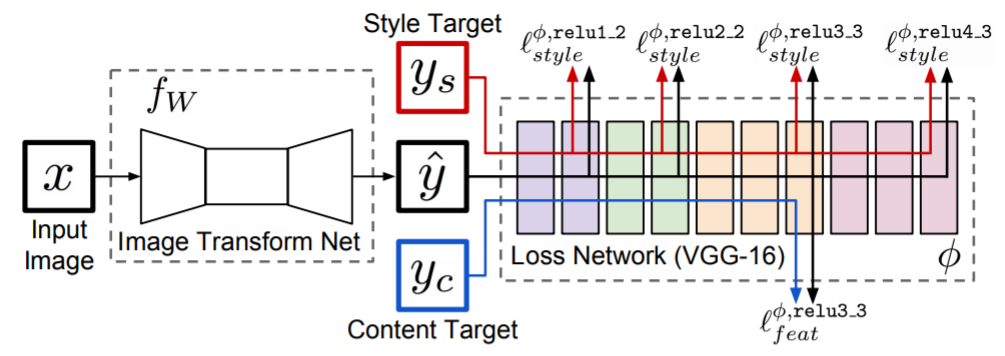
\includegraphics[width=0.79\textwidth]{resources/content/fast_neural_style.png}
        \caption{Trainingsprozess eines Image Transformer Networks \cite{DBLP:journals/corr/JohnsonAL16}}
        \label{img:fast_neural_style_transfer}
    \end{figure}
\end{frame}

\begin{frame}
    \frametitle{Perceptual Losses for Real-Time Style Transfer and Super-Resolution \cite{DBLP:journals/corr/JohnsonAL16}}

    Kombination aus unterschiedlichen Layer-Blöcken.
    
    \pause

    \begin{figure}[H]
        \centering
        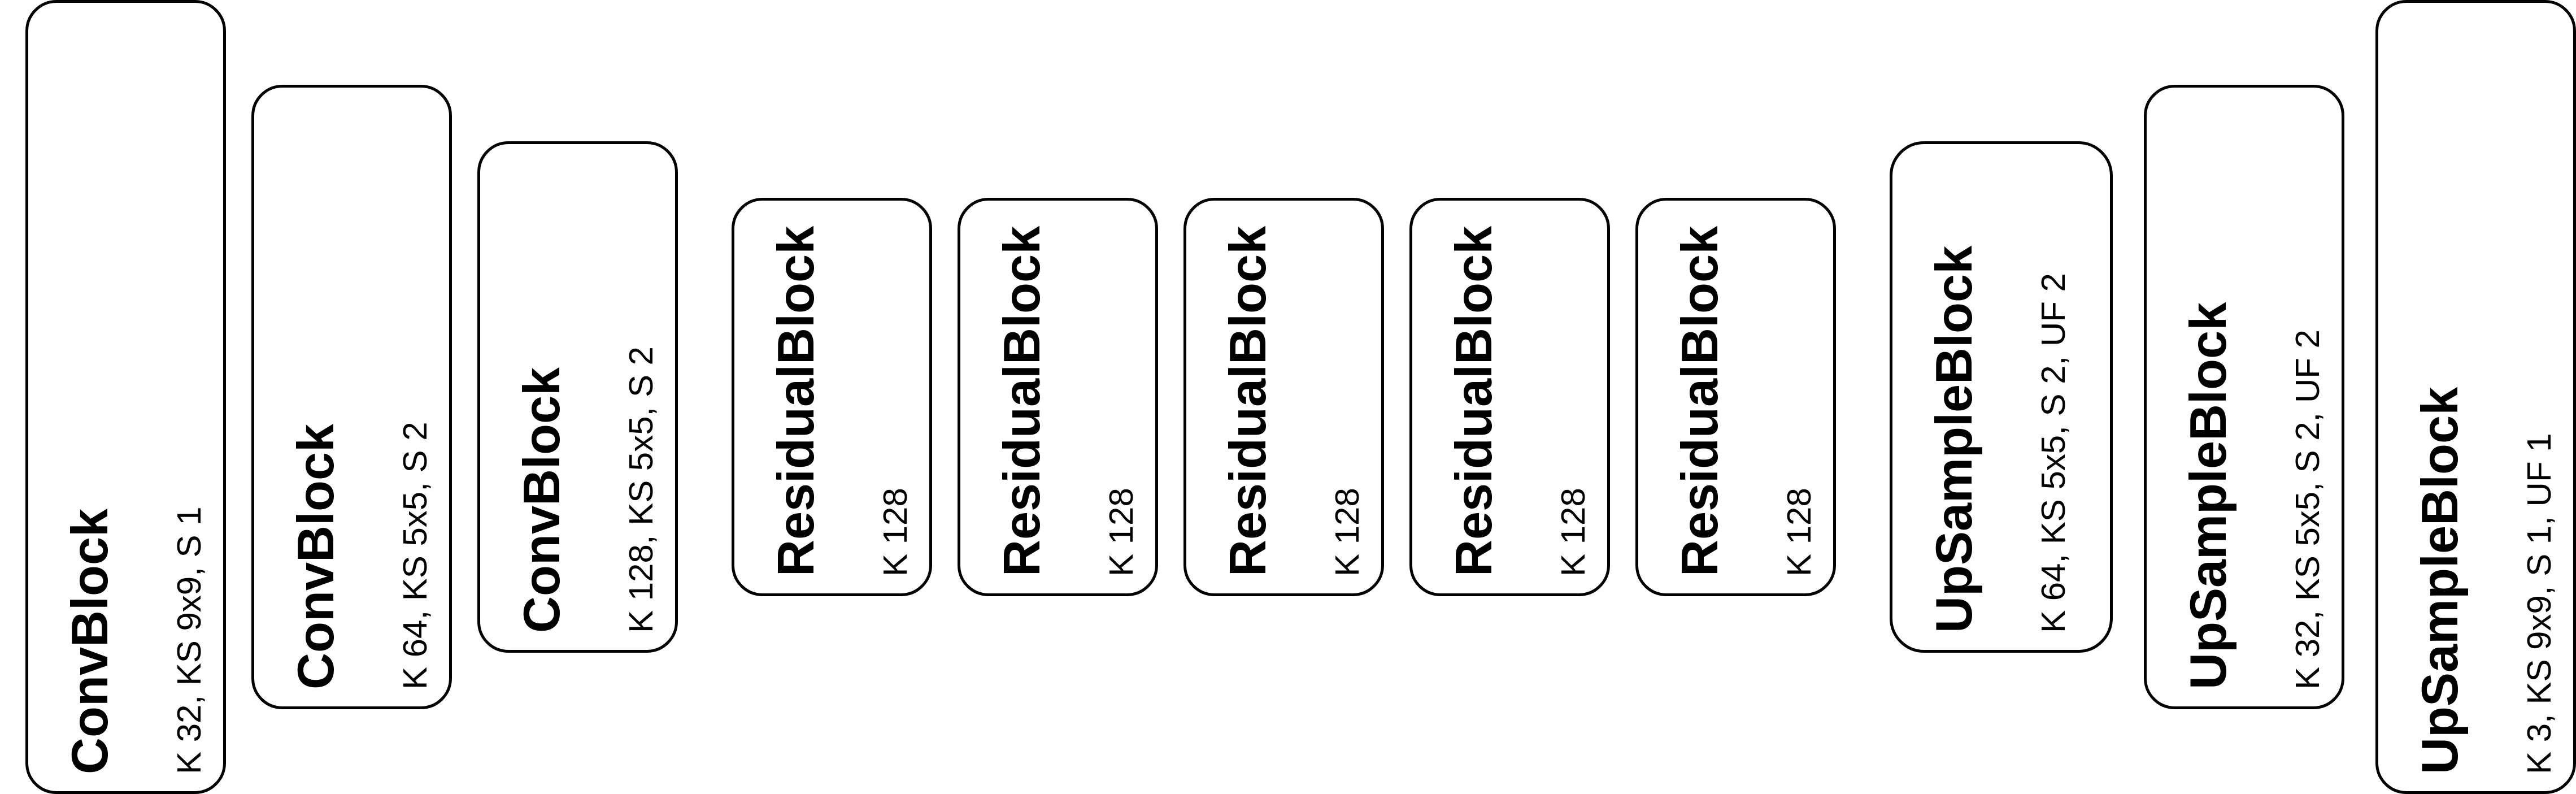
\includegraphics[width=1.0\textwidth]{resources/content/transformer_net.png}
        \caption{Netzwerkarchitektur des Transformer Net, eigene Darstellung}
        \label{img:transformer_net_img}
    \end{figure}    
\end{frame}

\begin{frame}
    \frametitle{Perceptual Losses for Real-Time Style Transfer and Super-Resolution \cite{DBLP:journals/corr/JohnsonAL16}}

    Definition  zwei neuer Variablen:

    \begin{itemize}
        \item Multiplikator $ m $: Multiplikator für die Anzahl der verwendeten Kernel der Convolutions im Netzwerk
        \item Bottleneck-Size $ s $: Anzahl der ResidualBlocks im Bottleneck-Teil
    \end{itemize}
\end{frame}



